\chapter{On the historical development of regularizers}%
\label{chap:regularizers}%
\graphicspath{{chapters/regularizers/scripts}}%
In \marginnote{\footnotesize \textbf{Contents:}\\\localtableofcontents}this chapter we outline the historical development of regularizers, starting with classical variational penalties such as magnitude or \gls{tv} penalties.
\gls{tv} regularization finds motivation in the histograms of natural images responses on finite difference filters, where the absolute value provides the best convex fit to the negative log-histograms.
This immediately suggests a generalization of this model:
a suitable set of filters, which can be readily computed from a set of reference images, is given by the principal directions of all image patches extracted from the reference images.
When sacrificing convexity, suitable potential functions are derived from the corresponding negative log-histograms.

However, despite their effectiveness in \gls{map} inference, these models do not account for the nontrivial correlation of overlapping patches, making them a bad model for the reference density.
In contrast, \gls{mrf} modeling accounts for this correlation.
By explicitly imposing translation invariance via convolutions, such models become very parameter efficient at the cost of a much more complex learning problem.
The \gls{pogmdm} discussed in~\cref{chap:pogmdm} exemplifies this approach.
Finally, the deep neural regularizer discussed in~\cref{chap:deep neural regularizers} models the reference density through a general map provided by a deep neural network.
Although sacrificing some interpretability and presenting an even more challenging learning problem, these models demonstrate excellent performance.

\section{A running example from MRI reconstruction}
To illustrate the historical development of regularizers, we employ a running example from \gls{mri} reconstruction.
However, the core focus of this chapter lies in examining \emph{the effect of the choice of the regularizer}.
For this purpose, we consider a simple reconstruction problem using synthetic data.
In contrast, much of \cref{chap:deep neural regularizers} is dedicated to developing clinically relevant reconstruction algorithms for real data.

We aim to reconstruct an image from Fourier data \( \Data \in \C^{f} \) constructed as
\begin{equation}
	\Data = \Mask \Fourier_{\R}\Signal + \Noise \coloneqq \Forward\Signal + \Noise,
\end{equation}
where \( x \in \R^{\Height \times \Width} \) represents the reference signal.
The two-dimensional \enquote{real} Fourier transform \( \map{\Fourier_{\R}}{\R^{\Height \times \Width}}{\C^{\Height \times (\lfloor \Width / \num{2} \rfloor + \num{1})}} \) exploits conjugate symmetry of the Fourier transform for real-valued signal by storing only half of the frequency plane.
Additionally, the Fourier transform is \emph{orthonormal}, i.e. that \( \Fourier_{\R}\Adjoint{\Fourier_{\R}} = \Adjoint{\Fourier_{\R}}\Fourier_{\R} = \Identity \).
The frequency selection operator\footnote{
	Other names for this object include \emph{undersampling mask} and \emph{subsampling-} or \emph{downsampling operator}.
} \( \map{\Mask}{\C^{\Height \times (\lfloor \Width / \num{2} \rfloor + \num{1})}}{\C^{f}} \) is a binary diagonal operator that selects \( f \in \mathbb{N} \) frequencies, simulating the \emph{acceleration} in clinical \gls{mri} systems (details in \cref{chap:deep neural regularizers}).
\( \Forward \) is a shorthand for \( \Mask\Fourier_{\R} \).

In this chapter, the reference signal \( x \) is the root-sum-of-squares reconstruction of an \gls{mri} scan in the fastMRI~\cite{zbontar_fastmri_2018} data set.\footnote{%
	It is the \num{17}-th slice in the file \texttt{file1000005.h5} folder \texttt{multicoil\_train}.%
}
The images in the fastMRI dataset are square with size \( m = n = \num{320} \).
\RunningExampleFigure{reference-rss}{Reference signal}{The reference signal used throughout this chapter.}
\begin{sidefigure}
	\centering
	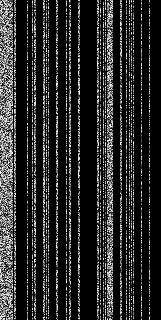
\includegraphics[width=2cm]{log-abs-data}
	\caption[Running example: Zero-filled data]{%
		The logarithm of the absolute value of the zero filled data \( \Adjoint{\Mask}\Data \).
	}%
	\label{fig:running example data}
\end{sidefigure}
\Cref{fig:running example reference-rss} and~\cref{fig:running example data} depict the reference signal and the data respectively.
In order to visualize the data \( y \), we map it back to \( \C^{\Height \times (\lfloor \Width / \num{2} \rfloor + \num{1})} \) using \( \Adjoint{\Mask} \).

This chapter is dedicated to finding
\begin{equation}
	\argmin_{x \in \R^{\Height \times \Width}} \Half \norm{\Forward\Signal - \Data}_{\num{2}}^{\num{2}} + R(x)
	\label{eq:running example optimization problem}
\end{equation}
under varying choices of \( R \).
To underscore the significance of the choice of \( R \), we initially set \( R \equiv 0 \).
Consequently, the least squares problem \( \argmin_{x \in \R^{\Height \times \Width}} \{ f(x) \coloneqq \Half \norm{\Forward\Signal - \Data}^{\num{2}} \} \) has the (not necessarily unique) solution \( \Adjoint{\Forward}\Data \).
This can be seen by noting that Fermat's condition (\cref{th:fermat}) at \( \Adjoint{\Forward}\Data \),
\begin{equation}
	\Grad f(\Adjoint{\Forward} \Data) = \Adjoint{\Forward}(\Forward\Adjoint{\Forward}\Data - \Data) = 0,
\end{equation}
is fulfilled since \( \Forward\Adjoint{\Forward} = \Mask\Fourier_{\R}\Adjoint{\Fourier_{\R}}\Adjoint{\Mask} = \Identity \) (on \( \C^f \)).
This solution is commonly referred to as the \emph{zero-filling} solution, as \( \Adjoint{\Forward} y = \Adjoint{\Fourier_{\R}}\Adjoint{\Mask}y \) essentially fills the missing frequencies with \num{0} before inverting the Fourier transform.
The reconstruction in~\cref{fig:running example reconstructions/zero-filled} shows the classical back-folding artifacts as well as high-frequency noise.
\RunningExampleFigure{reconstructions/zero-filled}{Naive reconstruction}{Zero-filling solution \( \Adjoint{\Fourier_{\R}}\Adjoint{\Mask}y \).}

\section{Classical variational penalties}
As the first interesting choice for \( R \), we consider the quadratic two-norm \( \frac{\lambda}{2} \norm{}^{\num{2}} \), where \( \lambda > 0 \).
Under this choice of \( R \), the first order optimality conditions of~\cref{eq:running example optimization problem} lead to the unique solution
\begin{equation}
	\Optimal{\Signal} = (\Adjoint{\Forward} \Forward + \lambda\Identity)^{-1} \Adjoint{\Forward}\Data,
\end{equation}
where the existence of the inverse of the operator \( \Adjoint{\Forward} \Forward + \lambda \Identity \) is assured by construction.

This regularization is extremely popular in many applications;
for instance, in machine learning applications it is called \emph{weight decay}~\cite[section 5.2.2, section 7.1.1]{goodfellow_deeplearning_2016}.
In the Bayesian framework adopted in this thesis, it corresponds to the assumption that the underlying signal is normally distributed with mean zero.
In imaging applications, this is typically not useful as it biases the solution towards dark images.
It enforces \enquote{regularity} solely on the magnitude of pixel intensities, irrespective of their neighbourhood, making in invariant with respect to arbitrary permutations of the pixels.
This characteristic is undesirable for regularizers of images, which have inherent spatial ordering.
\RunningExampleFigure{reconstructions/quadratic-intensities}{Quadratic intensity penalization}{Reconstruction using quadratic pixel magnitude penalization.}

For our forward operator, the inverse of \( \Adjoint{\Forward} \Forward + \lambda \Identity \) can be calculated quickly by noting that \( (\Adjoint{\Fourier_{\R}}\Adjoint{\Mask} \Mask\Fourier_{\R} + \lambda \Identity)^{-1} = (\Adjoint{\Fourier_{\R}}\Adjoint{\Mask} \Mask\Fourier_{\R} + \lambda \Adjoint{\Fourier_{\R}} \Fourier_{\R})^{-1} = (\Adjoint{\Fourier_{\R}}(\Adjoint{\Mask} \Mask + \lambda \Identity)\Fourier_{\R})^{-1} = \Adjoint{\Fourier_{\R}}(\Adjoint{\Mask} \Mask + \lambda \Identity)^{-1}\Fourier_{\R} \) where \( \Adjoint{\Mask}\Mask \) is a diagonal operator containing only ones and zeros.
Therefore, we have
\begin{equation}
	\begin{aligned}
		\Optimal{\Signal} &= \Adjoint{\Fourier_{\R}}(\Adjoint{\Mask} \Mask + \lambda \Identity)^{-1}\Fourier_{\R} \Adjoint{\Fourier_{\R}}\Adjoint{\Mask}\Data \\
						  &= \Adjoint{\Fourier_{\R}}(\Adjoint{\Mask} \Mask + \lambda \Identity)^{-1}\Adjoint{\Mask}\Data \\
						  &= (\num{1} + \lambda)^{-1}\Adjoint{\Fourier_{\R}}\Adjoint{\Mask}y,
	\end{aligned}
\end{equation}
where the last equality holds since \( \Adjoint{\Mask}\Data \) is only non-zero in entries whose corresponding position in the diagonal operator \( \Adjoint{\Mask} \Mask + \lambda \Identity \) are \( 1 + \lambda \).
In other words, the reconstruction shown in~\cref{fig:running example reconstructions/quadratic-intensities} is just the zero-filling solution multiplied by \( (1 + \lambda)^{-1} \).

Instead of penalizing the magnitude of pixel intensities, a fruitful approach is to penalize\footnote{%
	The regularizers we consider in these sections generally penalize responses.
	Later in~\cref{sec:overcompleteness through convolution} we discuss regularizers where this is not necessarily true.
} responses to linear filters.
Regularizers of this type can in general be represented as
\begin{equation}
	x \mapsto \lambda \sum_{i,j=\num{1}}^{m,n} \sum_{k=\num{1}}^{\NumExperts} \Potential_k\bigl((K_k x)_{i,j}\bigr).
	\label{eq:ridge regularizers}
\end{equation}
Here, \( \map{K_{\num{1}}, K_{\num{2}}, \dotsc, K_{\NumExperts}}{\R^{\Height \times \Width}}{\R^{\Height \times \Width}} \) are convolution operators (\cref{ssec:convolutions}) and \( \map{\Potential_{\num{1}}, \Potential_{\num{2}}, \dotsc, \Potential_{\NumExperts}}{\R}{\R} \) are scalar functions.

In this thesis, we adopt the nomenclature from the \gls{mrf} literature, see e.g.~\cite{geman_stoch_84,RoBl09,zhu_minimax_1997,zhu_filters_1998}.
Each operator \( K_k \) is endowed with its own \emph{potential} \( \Potential_k \), which is applied to the \emph{filter responses}.
In terms of the statistical model where the regularizer is interpreted as the negative log-prior, the regularizer encodes a \emph{Gibbs distribution}~\cite[theorem 1 and the two preceding definitions]{zhu_filters_1998} with density
\begin{equation}
	x \mapsto Z(K_{\num{1}}, \Expert_{\num{1}}, K_{\num{2}},\Expert_{\num{2}}, \dotsc, K_\NumExperts,\Expert_\NumExperts)^{\num{-1}} \prod_{i,j=\num{1}}^{\Height, \Width} \prod_{k=\num{1}}^\NumExperts \Expert_k\bigl( (K_kx)_{i, j} \bigr).
\end{equation}
Here, analogous to the products-of-experts model from Hinton~\cite{hinton_training_2002}, the one-dimensional functions \( \map{\Expert_{\num{1}}, \Expert_{\num{2}}, \dotsc, \Expert_\NumExperts}{\R}{\R} \) are termed \emph{experts}.
Thus, the potential \( \Potential_k \) is related to the expert \( \Expert \) via \( \Potential_k = -\log \Expert_k \).
The gradient of the potential function is called the \emph{activation}.\footnote{This is borrowed from the neural network literature.}
\( Z \) is the \emph{partition function} such that the density is normalized.

A simple choice for the convolution operators is \( \map{K_{\num{1}} = \DiffOp_h, K_{\num{2}} = \DiffOp_v}{\R^{\Height \times \Width}}{\R^{\Height \times \Width}} \), where \( \DiffOp_h \) and \( \DiffOp_v \) are discretizations of horizontal and vertical image gradients, respectively.
A standard choice~\cite{chambolle_algorithm_2004,chambolle_primal_2010,chambolle_pock_2016_acta_numerica} for defining these operators is through forward finite differences with Neumann boundary conditions,
\begin{equation}
	\begin{aligned}
		(\DiffOp_v x)_{i, j} &= \begin{cases}
			x_{i + \num{1},j} - x_{i,j} & \text{if } \num{1} \leq i < \Height, \\
			0 & \text{else},
		\end{cases}\\
		(\DiffOp_h x)_{i, j} &= \begin{cases}
			x_{i,j + \num{1}} - x_{i,j} & \text{if } \num{1} \leq j < \Width, \\
			0 & \text{else}.
		\end{cases}
	\end{aligned}
\end{equation}
This choice is popular due to its simplicity but there exist many other discretizations.
However, the choice of discretization rarely matters in applications~\cite{chambolle_upwind_2011} and we adopt the forward finite differences scheme.
For ease of notation, we define a linear operator \( \map{D}{\R^{\Height \times \Width}}{\R^{\Height \times \Width \times \num{2}}} \) that summarizes the application of \( D_v \) and \( D_h \) via
\begin{equation}
	(\DiffOp x)_{i, j, \num{1}} = (\DiffOp_v x)_{i, j}\ \text{and}\ (\DiffOp x)_{i, j, \num{2}} = (\DiffOp_h x)_{i, j}.
\end{equation}

When the potentials are shared and chosen as \( \Potential_{\num{1}} = \Potential_{\num{2}} = (x \mapsto x^{\num{2}}/{\num{2}}) \), the resulting regularizer can be compactly written as
\begin{equation}
	x \mapsto \frac{\lambda}{2} \sum_{i,j=\num{1}}^{\Height,\Width} \sum_{k=\num{1}}^{\num{2}} \bigl( (\DiffOp x)_{i,j,k} \bigr)^{\num{2}} = \tfrac{\lambda}{2} \norm{Dx}_{\num{2}, \num{2}}^{\num{2}}.
	\label{eq:quadratic gradient penalization}
\end{equation}
Here, the subscript in the norm emphasizes that we take a two-norm over both the pixel- and gradient dimensions.
This regularizer encodes the assumption that image gradients have Gaussian marginal distributions.

The corresponding optimization problem
\begin{equation}
	\argmin_{\Signal \in \R^{\Height \times \Width}} \Half \norm{\Forward\Signal - \Data}_{\num{2}}^{\num{2}} + \tfrac{\lambda}{2}\norm{\DiffOp\Signal}_{\num{2},\num{2}}^{\num{2}}
\end{equation}
can again be solved in closed form as
\begin{equation}
	\Optimal{\Signal} = (\Adjoint{\Forward}\Forward + \lambda \Adjoint{\DiffOp}\DiffOp)^{-1}\Adjoint{\Forward}\Data.
\end{equation}
The operator \( \Adjoint{\Forward}\Forward + \lambda \Adjoint{\DiffOp}\DiffOp \) is invertible when \( \ker(\Forward) \cap \ker(\DiffOp) = \Set{0} \).
Without going into too much detail, this condition is fulfilled as long as \( \Mask \) captures the DC-component of the signal, since \( \ker(\DiffOp) = \Set{\text{constant signals in}\ \R^{\Height \times \Width}} \).
However, to avoid storing the operator in memory we utilize Nesterov's accelerated gradient method (\cref{alg:nesterovs accelerated gradient method}) to solve the optimization problem.
To ensure convergence, we choose the step size sequence \( \tau^k = (\num{1} + \lambda\norm{\DiffOp}^{\num{2}})^{-1} \) using \(\sqrt{\num{8}} \) as an upper bound for \( \norm{D} \) from~\cite{chambolle_algorithm_2004}.

In the resulting reconstruction in~\cref{fig:running example reconstructions/quadratic-gradients}, some back-folding artifacts are removed, and the image appears less noisy than previous reconstructions.
However, edges appear overly smooth and small details such as the blood vessels in the fat tissue are almost completely lost.
This is because the quadratic potentials poorly match the empirical marginal distributions of edges in natural images.
\RunningExampleFigure{reconstructions/quadratic-gradients}{Quadratic gradient penalization}{Reconstruction using quadratic gradient penalization.}

It has been known at least since 1999 that the empirical marginal distributions of edges in natural images are highly non-Gaussian~\cite{hua_statistics_1999}.
This is illustrated in~\cref{fig:edge histograms}, which shows the empirical negative log-histograms of edges in natural images.
\begin{sidefigure}
	\def\aaa{80}
	\def\bbb{30}
	\def\ccc{18}
	\centering
	\begin{tikzpicture}
        \begin{axis}[
			height=4.6cm,
			width=4.6cm,
			xmin=-0.4,
			xmax=0.4,
			no markers,
			grid=major,
			table/col sep=comma,
			marginlabels,
        ]
			\addplot [maincolor, thick] table{./chapters/regularizers/scripts/edge-statistics/d_h.csv};
			\addplot [samples=100, domain=-.4:.4, dashed, thick] {\aaa*pow(x, 2) - 16.0};
			\addplot [samples=100, domain=-.4:.4, thick] {\bbb*abs(x) - 16.0};
		  \end{axis}
	\end{tikzpicture}
	\caption[Histograms of edges in natural images and approximations with convex functions]{%
		\tikzexternaldisable
		Negative log-histogram of horizontal edges in natural images %
		\protect\tikz[baseline=-\the\dimexpr\fontdimen22\textfont2\relax]\protect\draw [maincolor, thick] (0,0) -- (.5, 0);. %
		The quadratic %
		\protect\tikz[baseline=-\the\dimexpr\fontdimen22\textfont2\relax]\protect\draw [dashed, thick] (0,0) -- (.5, 0);, and absolute potentials %
		\protect\tikz[baseline=-\the\dimexpr\fontdimen22\textfont2\relax]\protect\draw [thick] (0,0) -- (.5, 0); %
		correspond to the choices in~\cref{eq:quadratic gradient penalization} and~\cref{eq:absolute gradient penalization} respectively.%
		\tikzexternalenable
	}%
	\label{fig:edge histograms}
\end{sidefigure}
These empirical marginal distributions are highly leptokurtic (\cref{def:excess kurtosis platykurtic mesokurtic leptokurtic}).
Huang and Mumford report an excess kurtosis of more than \num{14} in~\cite{hua_statistics_1999}.
Additionally, there is a very sharp peak at zero, indicating that the vast majority of edges in natural images are very close to zero.
Simultaneously, edges with large magnitude occur much more often than would be expected under a Gaussian distribution.
This \emph{sparsity} of edges in natural images is demonstrated in~\cref{fig:gradient sparsity of natural images}.
\begin{sidefigure}
	\centering
	\begin{tikzpicture}
		\begin{scope}
			\clip (-2, 2) -- (2, 2) -- (-2, -2) -- cycle;
			\node [anchor=center, rotate=180] at (0, 0) {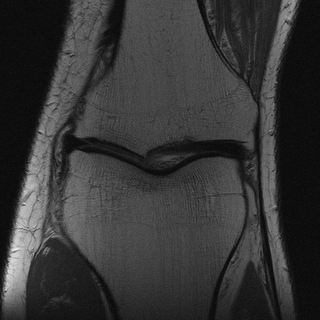
\includegraphics[width=4cm]{reference-rss}};
		\end{scope}
		\begin{scope}
			\clip (2, 2) -- (-2, -2) --(2, -2) -- cycle;
			\node [anchor=center, rotate=180] at (0, 0) {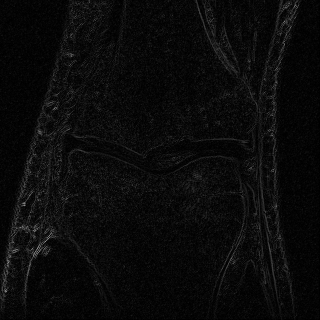
\includegraphics[width=4cm]{dx}};
		\end{scope}
	\end{tikzpicture}
	\caption[Sparsity of edges in natural images]{%
		Sum of the absolute horizontal and vertical difference of neighboring pixels (bottom right) of an \gls{mri} image from the fastMRI~\cite{zbontar_fastmri_2018} dataset (top left).
	}%
	\label{fig:gradient sparsity of natural images}
\end{sidefigure}

The analysis of the negative log-marginal distributions of edges in natural images (\cref{fig:edge histograms}) suggests considering other potential functions that match these more closely.
Among convex functions, the absolute value is best approximates the negative log-marginal distributions of edges.
Choosing \( \Potential_{\num{1}} = \Potential_{\num{2}} = \abs{} \) leads to the well known anisotropic \gls{tv} regularizer
\begin{equation}
	x \mapsto \lambda \sum_{i,j=\num{1}}^{m,n} \sum_{k=\num{1}}^{\num{2}} \abs*{(\DiffOp x)_{i,j,k}} = \lambda \norm{Dx}_{\num{1}, \num{1}}.
	\label{eq:absolute gradient penalization}
\end{equation}
Again, we adopt this simple interpretation of the discrete anisotropic \gls{tv} but point out that there exists a large literature on more elaborate, even learned (with respect to approximating some continuous energy), discretizations~\cite{bogensperger_learned_2023,chambolle_learning_2021,condat_tv_2017}.
Here, \emph{anisotropic} emphasizes that this regularizer favors grid-aligned edges.
We discuss different versions of the discrete \gls{tv} in~\cref{ssec:tv}.

The one-norm is a highly popular sparsity-inducing function~\cite{Daubechies2004,unser_representer_2016}.
There are many ways to see the sparsity-inducing property of the one-norm, such as the classical \enquote{intersection of level lines} in~\cite[figure 3.11]{Hastie2009} or by observing that its proximal map (\cref{def:proximal operator}) sets all elements smaller than a threshold to zero (see~\cref{fig:soft shrinkage}).
However, from the Bayesian perspective adopted in this thesis, the prior assumptions on the underlying signal are \emph{not} that \( Dx \) is sparse:
Although the \gls{map} solution favors sparse edges, samples from the Laplace distribution are never zero, e.g.\ see~\cite[fig. 1]{adler_deep_2018} for samples from a \gls{tv} prior.

This discrepancy is summarized by the difference between \emph{penalized likelihood estimation}, and \emph{Bayesian estimation}~\cite{bohra_phdthesis,gribonval_penalized_2011}.
In the former, the reconstructed signal has some abstract desirable regularity properties (like sparse edges), but the corresponding probabilistic model is in general \emph{not} a \enquote{good} model of the underlying distribution.
In the latter, the aim is to construct a good probabilistic model of the underlying distribution, whose corresponding \gls{map} estimate might not necessarily exhibit these abstract desirable regularity properties.
An illustrative example is~\cref{fig:gradient sparsity of natural images}: At almost all pixels, the sum of the absolute horizontal and vertical edges is almost zero.
Thus, we derive the abstract property that the underlying signal has sparse gradients.
However, a numerical check reveals that actually at exactly \emph{zero} pixels the sum of the absolute horizontal and vertical edges is \emph{exactly} zero.\footnote{%
	This has been checked on a \qty{32}{\bit} representation of the normalized image (maximum pixel intensity of \num{1}) with a threshold of \num{1e-7}.
	Only two pixels have a value lower than \num{1e-6}.
}
We refer to the papers of Gribonval et al.~\cite{gribonval_penalized_2011,gribonval_compressible_2012} for other Bayesian interpretations of penalized likelihood estimators and to the thesis of Bohra~\cite[section 2.2]{bohra_phdthesis} for a slightly more in-depth discussion.

Optimizing~\cref{eq:running example optimization problem} under the choice of \( R \) in~\cref{eq:absolute gradient penalization} is challenging because the absolute value is not differentiable.
This can be overcome by using differentiable surrogate functions such as \( x \mapsto \sqrt{x^{\num{2}} + \epsilon^{\num{2}}} \) or \( x \mapsto \epsilon^{-1}\log \cosh(\epsilon x) \) where \( \epsilon > \num{0} \)~\cite{chambolle_recovery_1997,charbonnier_deterministic_1997,charbonnier_deterministic_1994}.
The first choice was used by Charbonnier in 1994~\cite{charbonnier_deterministic_1994};
we use this differentiable surrogate in~\cref{chap:deep neural regularizers} for the isotropic \gls{tv} (see~\cref{ssec:tv}).
Another popular surrogate is the Huber function
\begin{equation}
	x \mapsto \begin{cases}
		x^{\num{2}} / \num{2} & \text{ if } \abs{x} \leq \epsilon, \\
		\epsilon(\abs{x} - \epsilon/\num{2}) & \text{ else},
	\end{cases}
\end{equation}
which we already introduced in~\cref{eq:huber function} as the Moreau envelope (\cref{def:moreau envelope}) of the absolute value.
\Cref{fig:absolute value and smooth variants} shows these surrogates for \( \epsilon = \num{1} \).
\begin{sidefigure}
	\begin{tikzpicture}
		\begin{axis}[%
			domain=-3:3,
			width=5cm,
			marginlabels,
			samples=200,
		]
			\addplot+{abs(x)};
			\addplot+{huber(x,1)};
			\addplot+{sqrt(pow(x, 2) + 1)};
			\addplot+{ln(cosh(x))};
		\end{axis}
	\end{tikzpicture}
	\caption[The absolute value and smooth surrogates]{%
		\tikzexternaldisable
		The absolute value %
		\protect\tikz[baseline=-\the\dimexpr\fontdimen22\textfont2\relax]\protect\draw [index of colormap={0} of flare, thick] (0,0) -- (.5, 0);
		and popular smooth surrogates:
		The Huber function %
		\protect\tikz[baseline=-\the\dimexpr\fontdimen22\textfont2\relax]\protect\draw [index of colormap={4} of flare, thick] (0,0) -- (.5, 0);,
		\( \sqrt{(\argm)^{\num{2}} + \num{1}} \) %
		\protect\tikz[baseline=-\the\dimexpr\fontdimen22\textfont2\relax]\protect\draw [index of colormap={8} of flare, thick] (0,0) -- (.5, 0);,
		and \( \log \circ \cosh \)
		\protect\tikz[baseline=-\the\dimexpr\fontdimen22\textfont2\relax]\protect\draw [index of colormap={12} of flare, thick] (0,0) -- (.5, 0);.
		\tikzexternalenable
	}%
	\label{fig:absolute value and smooth variants}
\end{sidefigure}

Using these approximations, we lose the interpretation of gradient \emph{sparsity}, since these functions are not sparsity-inducing (only \enquote{small value} inducing) and only approach the absolute value as \( \epsilon \) approaches zero.
As they approach the absolute value, the Lipschitz constant (\cref{def:lipschitz continuity}) of the their gradient necessarily has to explode.
This affects optimization algorithms since the step size (and hence the convergence speed) is bounded by the reciprocal of the Lipschitz constant of the gradient.

To achieve fast convergence even in the nondifferentiable case, we use primal-dual optimization algorithms.
Since the one-norm is a proper closed and convex function, it is equal to its biconjugate, see~\cref{th:biconjugate of convex function is itself}.
Thus, we can write
\begin{equation}
	\lambda \norm{x}_{\num{1},\num{1}} = (\Biconjugate{(\lambda\norm{}_{\num{1},\num{1}})})(x) = \max_{w \in \R^{\Height \times \Width \times \num{2}}} \inprod{w}{x} - (\ConvexConjugate{(\lambda \norm{}_{\num{1},\num{1}})})(w).
\end{equation}
The conjugate of the one-norm is the indicator function of the closed unit infinity-norm ball, see~\cref{th:convex conjugate of any norm}.
Additionally, we use~\cref{th:convex conjugate under postitive scaling} to identify
\begin{equation}
	\ConvexConjugate{(\lambda \norm{}_{\num{1},\num{1}})} = \lambda\IndicatorFunction{\Closure{\Ball{\norm{}_{\infty,\infty}}{\num{0}}{\num{1}}}}(\argm/\lambda) = \IndicatorFunction{\Closure{\Ball{\norm{}_{\infty,\infty}}{\num{0}}{\lambda}}},
\end{equation}
since indicator functions are invariant with respect to scaling and the scaling of the argument can be absorbed into the radius of the norm ball.
Thus,
\begin{equation}
	\lambda \norm{x}_{\num{1},\num{1}} = \max_{w \in \R^{\Height \times \Width \times \num{2}}} \inprod{w}{x} - \IndicatorFunction{\Closure{\Ball{\norm{}_{\infty,\infty}}{0}{\lambda}}}(w).
\end{equation}

The saddle point formulation of the optimization problem~\cref{eq:running example optimization problem} with the regularizer \( R \) being~\cref{eq:absolute gradient penalization} is
\begin{equation}
	\min_{\Signal \in \R^{\Height \times \Width}} \max_{w \in \R^{\Height \times \Width \times \num{2}}} \Half \norm{\Forward\Signal - \Data}_{\num{2}}^{\num{2}} + \inprod{w}{\DiffOp\Signal} +  \IndicatorFunction{\Closure{\Ball{\norm{}_{\infty,\infty}}{0}{\lambda}}}(w).
\end{equation}
This follows the structure~\cref{eq:primal dual saddle point structure} and we can use the \gls{pdhg} algorithm~(\cref{alg:pdhg},~\cite{chambolle_primal_2010}) to solve it efficiently.
In particular, the proximal map w.r.t.\ the indicator function is just a element-wise projection onto the interval \( \interval{-\lambda}{\lambda} \),
\begin{equation}
	w = \prox_{\IndicatorFunction{\Closure{\Ball{\norm{}_{\infty,\infty}}{0}{\lambda}}}}(\bar{w}) \iff w_{i,j,k} = \max(\min(\bar{w}_{i,j,k}, \lambda), -\lambda),
\end{equation}
and the proximal map w.r.t.\ the data fidelity term can be computed by
\begin{equation}
	\prox_{\tau\norm{\Forward\argm - \Data}_{\num{2}}^{\num{2}}/\num{2}}(x) = \Adjoint{\Fourier_{\R}}\bigl((\tau\Adjoint{\Mask}\Mask + \Identity)^{-1}(\Fourier_{\R} x + \tau\Adjoint{\Mask}\Data)\bigr).
	\label{eq:prox fourier data}
\end{equation}
There we used that \( \Adjoint{\Fourier_{\R}}\Fourier_{\R} = \Identity \) and note that \( \tau\Adjoint{\Mask}\Mask + \Identity \) is a diagonal operator that can be efficiently inverted.
In the algorithm, we used the standard choice \( \tau = \sigma = \frac{1}{\sqrt{8}} \).

The reconstruction in~\cref{fig:running example reconstructions/absolute-gradients} shows that back-folding artifacts are almost fully removed, the reconstruction has sharp edges, and some anatomical details are recovered.
\RunningExampleFigure{reconstructions/absolute-gradients}{Absolute gradient penalization}{Reconstruction using absolute gradient penalization, also known as the anisotropic total variation.}
However, it appears overly simplistic and fine anatomical structures such as the blood vessels in the fat tissue are almost entirely missing.
This simplification results from the simple model that only considers the distribution of differences between neighboring pixels and assumes these are independent random variables.

\Cref{fig:edge histograms} suggests nonconvex potential functions;
many have been proposed in the literature.
In \num{1985} Geman and McClure~\cite{geman_bayesian_1985} proposed the potential function
\begin{equation}
	x \mapsto -\bigl( \num{1} + (x / \gamma )^{\num{2}} \bigr)^{\num{-1}}
\end{equation}
where \( \gamma > \num{0} \) for photon emission tomography reconstruction.
Later, Huang and Mumford~\cite{hua_statistics_1999} considered the Student-t and generalized Laplace distributions.
The respective potential functions are
\begin{equation}
	x \mapsto \alpha \log \bigl( \num{1} + (x/\beta)^{\num{2}} \bigr)
\end{equation}
and
\begin{equation}
	x \mapsto \abs*{\frac{x}{\alpha}}^\beta
\end{equation}
where \( \alpha, \beta > \num{0} \) shape the potentials.
While these potentials better model the empirical marginal distributions of edges in natural images, the improvements over the absolute value are marginal.\footnote{;)}
\begin{sidefigure}
	\def\aaa{1.5}
	\def\bbb{0.01}
	\def\ccc{18}
	\centering
	\begin{tikzpicture}
		\begin{axis}[
			height=4.6cm,
			width=4.6cm,
			xmin=-0.4,
			xmax=0.4,
			no markers,
			grid=major,
			table/col sep=comma,
			marginlabels,
		]
			\addplot [maincolor, thick] table{./chapters/regularizers/scripts/edge-statistics/d_h.csv};
			\addplot [thick, samples=101, domain=-.4:.4] {\aaa * ln(1. + pow(x/\bbb, 2)) - 16};
			\addplot [thick, dashed, samples=101, domain=-.4:.4] {\ccc*sqrt(abs(x)) - 16};
		  \end{axis}
	\end{tikzpicture}
	\caption[Histograms of edges in natural images and approximations with nonconvex functions]{%
		\tikzexternaldisable
		The nonconvex Student-t %
		\protect\tikz[baseline=-\the\dimexpr\fontdimen22\textfont2\relax]\protect\draw [thick] (0,0) -- (.5, 0);
		and generalized Laplace potentials %
		\protect\tikz[baseline=-\the\dimexpr\fontdimen22\textfont2\relax]\protect\draw [dashed, thick] (0,0) -- (.5, 0);
		provide a good fit to the negative log-histograms of horizontal edges in natural images %
		\protect\tikz[baseline=-\the\dimexpr\fontdimen22\textfont2\relax]\protect\draw [maincolor, thick] (0,0) -- (.5, 0);.
		\tikzexternalenable
	}%
	\label{fig:edge histograms nonconvex functions}
\end{sidefigure}
\subsection{On the total variation}%
\label{ssec:tv}
In the previous section, we discussed \enquote{ridge-type} regularizers where a scalar potential function acts on filter responses and identified the discrete \emph{anisotropic} \gls{tv}
\begin{equation}
	x \mapsto \lambda \sum_{i,j=\num{1}}^{m,n} \sum_{k=\num{1}}^{\num{2}} \abs*{(\DiffOp x)_{i,j,k}} = \lambda \norm{Dx}_{\num{1}, \num{1}}
\end{equation}
as an instance of these models.
Here, isotropy is with respect to spatial directions, i.e.\ invariance with respect to rotations of the image.
Due to the definition of the forward finite difference operator \( \DiffOp \), this regularizer favors grid-aligned (horizontal and vertical) structures over oblique structures.
This anisotropy is essentially captured in~\cref{fig:norm balls}, where the one-norm ball is not radially symmetric.

To avoid these discretization artifacts, often the \emph{isotropic} \gls{tv}
\begin{equation}
	x \mapsto \lambda \sum_{i,j=\num{1}}^{m,n} \sqrt{\sum_{k=\num{1}}^{\num{2}} \bigl((\DiffOp x)_{i,j,k}\bigr)^{\num{2}}} = \lambda \norm{Dx}_{\num{2}, \num{1}}
\end{equation}
is employed.
There, the gradient \emph{magnitude} (as in the two-norm) is summed up over all pixels.
It turns out that the isotropic \gls{tv} is also anisotropic, see~\cite{condat_tv_2017}.
The isotropic \gls{tv} is not of the form~\cref{eq:ridge regularizers}, as the square root acts on the sum of the squares of the responses to two different filters, \( \DiffOp_v \) and \( \DiffOp_h \).
Thus, the isotropic \gls{tv} is in a more general class of regularizers.

The optimization of inverse problems with isotropic \gls{tv} regularization is usually performed with primal-dual methods similar to the anisotropic \gls{tv} discussed previously.
The associated saddle point problem problem is
\begin{equation}
	\min_{\Signal \in \R^{\Height \times \Width}} \max_{w \in \R^{\Height \times \Width \times \num{2}}} \Half\norm{\Forward\Signal - \Data}_{\num{2}}^{\num{2}} + \inprod{w}{\DiffOp\Signal} +  \IndicatorFunction{\Closure{\Ball{\norm{}_{\num{2},\infty}}{\num{0}}{\lambda}}}(w),
\end{equation}
which can be solved efficiently using \gls{pdhg} (\cref{alg:pdhg}).
The proximal map with respect to the indicator function is a pixel-wise projection onto two-norm balls with radius \( \lambda \),
\begin{equation}
	w = \prox_{\IndicatorFunction{\Closure{\Ball{\norm{}_{\num{2},\infty}}{\num{0}}{\lambda}}}}(\bar{w}) \iff w_{i,j} = \frac{\bar{w}_{i,j}}{\max(\num{1}, \norm{\bar{w}_{i,j}}_{\num{2}}/\lambda)}.
\end{equation}

\RunningExampleFigure{reconstructions/isotropic-tv}{Data-driven undercomplete regularizer}{%
	Reconstruction using the isotropic \gls{tv} regularizer (\qty{30.35}{\decibel}).
	The difference to the reconstruction obtained with anisotropic \gls{tv} (\cref{fig:running example reconstructions/absolute-gradients}) is almost negligible (\qty{30.32}{\decibel}).
}

For the image reconstruction problems considered in this thesis, the differences between the discretizations is largely irrelevant.
\Cref{fig:running example reconstructions/isotropic-tv} shows the reconstruction using the isotropic \gls{tv} which quantitatively improves the reconstruction from \qty{30.32}{\decibel} to \qty{30.35}{\decibel} in \gls{psnr} compared to the anisotropic \gls{tv}.
However, for more complex applications where the \gls{tv} is a building block, the choice of discretization can be crucial~\cite{chambolle_total_2018}.

In~\cref{chap:deep neural regularizers}, we require a smooth version of the \gls{tv} due to the structure of the optimization problems.
There, we use the isotropic \gls{tv} with the popular smoothing proposed by Charbonnier~\cite{charbonnier_deterministic_1994}.
In this case, the regularizer reads
\begin{equation}
	x \mapsto \lambda \sum_{i,j=\num{1}}^{m,n} \sqrt{\sum_{k=\num{1}}^{\num{2}} \bigl((\DiffOp x)_{i,j,k}\bigr)^{\num{2}} + \epsilon^{\num{2}}},
\end{equation}
where \( \epsilon > \num{0} \) controls the smoothness.
\section{Data-driven regularizers}
All regularizes discussed in the previous section were concerned with modeling the histograms of differences of neighboring pixels.
However, natural images are highly structured and the distribution of any pixel heavily depends on its neighbors.
Therefore, a good statistical model of images should take this structure into account.

Up to now, we have only considered first order forward finite difference filters with a receptive field of two pixels.
One way to account for the spatial structure in images is to use larger filters, where classical choices include derivative filters on different scales, Laplacian of Gaussian filters, and Gabor filters~\cite{zhu_prior_1997,zhu_filters_1998}.
However, it becomes increasingly difficult to choose the filters and model the potential functions manually.
A more feasible approach is to derive both the filters and the potential functions from data.
These types of models are called \emph{data-driven}.

The degree to which models of natural images are data-driven can vary greatly.
The regularizers discussed in the previous section are also in some sense data-driven:
We motivated different choices of potential functions via the empirical (\enquote{data-driven}) negative log-histogram of filter responses.
Generalizing this idea, we can derive the filters themselves within the framework described by
\begin{equation}
	x \mapsto \lambda \sum_{i,j=\num{1}}^{m,n} \sum_{k=\num{1}}^{\NumExperts} \Potential_k\bigl((K_k x)_{i,j}\bigr).
\end{equation}
To emphasize the image \emph{patches} in this formulation, we write this as
\begin{equation}
	x \mapsto \lambda \sum_{i, j=\num{1}}^{m, n} \sum_{k=\num{1}}^{\NumExperts} \Potential_k \bigl( \inprod{\Filter_k}{P_{i, j}x} \bigr).
	\label{eq:ridge regularizer 2}
\end{equation}
Here, the convolution operators \( K_{\num{1}}, K_{\num{2}}, \dotsc, K_\NumExperts \) implement the convolution with filters \( \Filter_{\num{1}}, \Filter_{\num{2}}, \dotsc, \Filter_\NumExperts \) of size \( b \times b \), and \( P_{i, j} \) extracts patches at pixel location \( (i, j) \) with appropriate boundary handling.
When treating overlapping patches as independent, it becomes evident that under the Bayesian interpretation that we adopt in this thesis, the above is a good model of the negative log-density of images when
\begin{equation}
	p \mapsto \lambda \sum_{k=\num{1}}^{\NumExperts} \Potential_k \bigl( \inprod{\Filter_k}{p} \bigr)
\end{equation}
is a good model of the negative log-density of image patches.
This independence assumption introduces a modeling error (except in the trivial case when \( b = \num{1} \)), which we address and resolve rigorously below.

A popular statistical model for image patches, which can be readily computed from a set of reference images, is given by the \gls{pca}~\cite{zoran_learning_2011}.
Following this idea, we plot the principal directions of all overlapping \( \numproduct{7x7} \) patches in the \num{300} images contained in the \gls{bsds}~\cite{martin_database_2001} training and validation data set\footnote{%
	We use the \gls{bsds} images here because they serve as training data in~\cref{chap:pogmdm}.
	The results would be similar for knee \glspl{mri}.
}
in~\cref{fig:pca of bsds patches}.
The principal directions associated with the largest singular value are low-frequency horizontal and vertical gradients.
As the singular value decreases, the filters obtain more and more high-frequency components.
Over all, the obtained filters closely resemble the basis images of the two-dimensional \gls{dct} and classical Gabor and Fourier filters.
For comparison, the basis images of the \gls{dct} are shown in~\cref{fig:discrete cosine transform basis}.
The observation that \gls{pca} of image patches recovers the \gls{dct} is related to the observation that the \gls{dct} is a good approximation of the Karhunen-Loève transform for stationary processes, as has been pointed out by Unser~\cite{unser_approximation_1984}.
\begin{figure*}
	\begin{tikzpicture}
		\csvreader[no head]{chapters/regularizers/scripts/pca/sigmas.txt}{1=\ssigma}{
			\pgfmathsetmacro{\component}{int(\thecsvrow-1)}
			\pgfmathsetmacro{\yy}{-int((\component)/12)*1.3}
			\pgfmathsetmacro{\xx}{mod((\component),12)*1.3}
			\node at (\xx, \yy-.65) {\tiny \( \num{\ssigma} \)};
			\node at (\xx, \yy) {\includegraphics[frame,width=1cm]{pca/directions/\component/d_\component}};
		}
		\draw [gray, thick, rounded corners] (-1.1cm, -4.8cm) rectangle (15.0cm, 0.7cm);
		\node at (-1.4cm, -2.05cm) [rotate=90] {Principal directions};
		\begin{scope}[xshift=-.5cm,yshift=-6.3cm]
			\begin{groupplot}[
				pogmdm group plot,
				group style={
					group size=12 by 4,
				},
				ymin=-17,
				ymax=-5,
				xmin=-.35,
				xmax=.35,
			]
				\pgfplotsforeachungrouped \component in {0, ..., 47}
				{
					\edef\tmp{%
						\noexpand\nextgroupplot%
						\noexpand\addplot [thick, maincolor] table[col sep=comma]{chapters/regularizers/scripts/pca/directions/\component/hist.csv};%
					}\tmp
				}
			\end{groupplot}
			\draw [gray, thick, rounded corners] (-0.6cm, -4.4cm) rectangle (15.5cm, 1.2cm);
			\node at (-0.9cm, -1.6cm) [rotate=90] {Empirical marginals};
		\end{scope}
	\end{tikzpicture}
	\caption[Principal directions of image patches]{%
		The principal directions of overlapping zero-mean patches extracted from natural images shown on top resemble the basis images of the \gls{dct} shown in~\cref{fig:discrete cosine transform basis}.
		The principal directions here are ordered by decreasing singular value shown below the directions; the last principal direction (which is the constant image) is omitted.
		On the bottom, the negative-log histogram of the filter responses is drawn.
	}%
	\label{fig:pca of bsds patches}
\end{figure*}
\begin{figure*}
	\begin{tikzpicture}
		\foreach \component in {0,...,48}
		{
			\pgfmathsetmacro{\yy}{-int((\component)/7)*1.2}
			\pgfmathsetmacro{\xx}{mod((\component),7)*1.2}
			\ifthenelse{\component=0}{}{\node at (\xx, \yy) {\includegraphics[frame,width=1cm]{dct/\component}};}
		}
	\end{tikzpicture}
	\caption[The basis images of the two-dimensional discrete cosine transform]{%
		The basis images of the two-dimensional \gls{dct}, in increasing horizontal frequency (left-to-right) and vertical frequency (top-to-bottom).
		The basis images are normalized such that they have a minimum and maximum of \num{-1} and \num{1} respectively; the first basis image (which is the constant image) is omitted.
	}%
	\label{fig:discrete cosine transform basis}
\end{figure*}

When the filters are aligned with the principal directions, it remains to detail the potential functions.
Since \gls{pca} provides an orthogonal basis, optimizing the potentials involves fitting each potentials to the corresponding observed negative log-marginal.
Using a suitable parametrization, such as piecewise constant functions~\cite{zhu_filters_1998} or radial basis functions~\cite{chen_trainable_2017}, this task becomes a least-squares fitting on the negative log-marginals.

The undercomplete model described in~\cref{chap:pogmdm} shares similarities these ideas, although the motivation is different.
This model also learns an orthogonal basis and parametrized potentials from a set of patches.
After training, the learned filters and potentials in~\cref{fig:learned patch reg} resemble the principal directions and negative log-marginals shown in~\cref{fig:pca of bsds patches}.
The negative log-marginals of the learned filters, shown in the bottom row of \cref{fig:learned patch reg}, closely match the learned potentials.
The shape of the learned negative log-marginals in \cref{fig:learned patch reg} remains consistent across all filters, while those of the principal directions in~\cref{fig:pca of bsds patches} appear \enquote{squashed} as the singular value decreases.
This difference is due to the choice of parametrization of the learned model where the filter norms change instead of the potentials being squashed.
The norm of the filters is related to the smallest and largest entry in the filter; these are shown below the filters in \cref{fig:learned patch reg}.
\begin{figure*}
	\centering
	\begin{tikzpicture}
		\csvreader[no head]{chapters/regularizers/scripts/ours/gmm/kvals.csv}{1=\kmin,2=\kmax}{
			\pgfmathsetmacro{\component}{int(\thecsvrow-1)}
			\pgfmathsetmacro{\yy}{-int((\component)/12)*1.3}
			\pgfmathsetmacro{\xx}{mod((\component),12)*1.3}
			\node at (\xx, \yy-.65) {\tiny \( \interval{\kmin}{\kmax} \)};
			\node at (\xx, \yy) {\includegraphics[frame,width=1cm]{ours/gmm/\component/k_\component}};
		}
		\draw [gray, thick, rounded corners] (-1.1cm, -4.8cm) rectangle (15.0cm, 0.7cm);
		\node at (-1.4cm, -2.05cm) [rotate=90] {Learned filters};
		\begin{scope}[xshift=-.5cm,yshift=-6.3cm]
			\begin{groupplot}[
				pogmdm group plot,
				group style={
					group size=12 by 4,
				},
				ymin=-3,
				ymax=8,
				xmin=-1,
				xmax=1,
				xticklabel=\empty,
			]
				\pgfplotsforeachungrouped \component in {0, ..., 47}
				{
					\edef\tmp{%
						\noexpand\nextgroupplot%
						\noexpand\addplot [thick, maincolor] table[col sep=comma, x=x, y=a]{chapters/regularizers/scripts/ours/gmm/\component/potentials.csv};%
					}\tmp
				}
			\end{groupplot}
			\draw [gray, thick, rounded corners] (-0.6cm, -4.1cm) rectangle (15.5cm, 1.2cm);
			\node at (-0.9cm, -1.6cm) [rotate=90] {Learned potentials};
		\end{scope}
		\begin{scope}[xshift=-.5cm,yshift=-11.9cm]
			\begin{groupplot}[
				pogmdm group plot,
				group style={
					group size=12 by 4,
				},
				ymin=-17,
				ymax=-5,
				xmin=-1,
				xmax=1,
			]
				\pgfplotsforeachungrouped \component in {0, ..., 47}
				{
					\edef\tmp{%
						\noexpand\nextgroupplot%
						\noexpand\addplot [thick, maincolor] table[col sep=comma,x=x,y=a]{chapters/regularizers/scripts/ours/gmm/\component/hists.csv};%
					}\tmp
				}
			\end{groupplot}
			\draw [gray, thick, rounded corners] (-0.6cm, -4.4cm) rectangle (15.5cm, 1.2cm);
			\node at (-0.9cm, -1.6cm) [rotate=90] {Empirical marginals};
		\end{scope}
	\end{tikzpicture}
	\caption[Learned directions and potential functions]{%
		A learned undercomplete model based on filter responses.
		The learned filters (top) share striking similarity to the \gls{pca} basis shown in~\cref{fig:pca of bsds patches}.
		The intervals below the filters show the value of black and white respectively.
		The learned potential functions (middle) match the negative-log empirical marginal distributions (bottom) almost perfectly.
		For more details, see~\cref{chap:pogmdm} and~\cite{zach_pogmdm_2024}.
	}%
	\label{fig:learned patch reg}
\end{figure*}

Due to the parametrization, the potential functions of this model are infinitely often differentiable but not convex, making the optimization problem~\cref{eq:running example optimization problem} smooth and non-convex.
Algorithms for solving these problems include \gls{ipiano} (see~\cref{alg:ipiano}) or non-convex \gls{fista} (see~\cref{alg:fista}).
We use the latter with a proximal step on the data fidelity which we recall from~\cref{eq:prox fourier data}, and determine the step sizes with backtracking~\cite{beck_fista_2009,ochs_ipiano_2014}.

The reconstruction using the learned regularizer\footnote{%
	The regularizer used to produce ~\cref{fig:running example reconstructions/patch-prior} is not exactly the one shown in~\cref{fig:learned patch reg}.
	Instead, to ease optimization we used the regularizer at diffusion time \( t = \num{5e-5}\), see~\cref{ssec:patch model}.%
} shown in~\cref{fig:running example reconstructions/patch-prior} appears more natural than the one using anisotropic \gls{tv} in \cref{fig:running example reconstructions/absolute-gradients}.
The back-folding artifacts are nearly eliminated and more details are retrieved without producing the staircasing artifacts associated with anisotropic \gls{tv}.
However, the reconstruction appears over-smoothed and important anatomical structures are missing.
In the next section, we discuss more expressive models that yield even better reconstructions.
\RunningExampleFigure{reconstructions/patch-prior}{Data-driven undercomplete regularizer}{Reconstruction using the undercomplete regularizer discussed in~\cref{chap:pogmdm}.}

\section{Overcomplete models and maximum entropy}%
\label{sec:overcompleteness through convolution}
In terms of the statistical model on the \emph{image}, the subtle but crucial assumption behind the previous models is the \emph{independence} of \emph{patches} at different pixel locations.
This introduces a modeling error, which we demonstrate with an example.
Consider three-by-three images where the marginal distribution of differences of neighboring pixels follow a normal distribution with unit variance.
Formally, let \( X \) be a random variable on \( \R^{\numproduct{3x3}} \) where
\begin{equation}
	(X_{i, j} - X_{i, j + \num{1}}) \sim \NormalDistribution_{\num{0},\num{1}}\ \text{for all}\ i = \numlist{1;2;3},\ \text{and}\ j=\numlist{1;2},
\end{equation}
and
\begin{equation}
	(X_{i, j} - X_{i + \num{1}, j}) \sim \NormalDistribution_{\num{0}, \num{1}}\ \text{for all}\ i = \numlist{1;2},\ \text{and}\ j=\numlist{1;2;3}.
\end{equation}
Using the approach from the previous sections where the density of \( X \) is modeled via the product of its marginals, we get
\begin{equation}
	\begin{aligned}
		&p_{\hat{X}}(x) \\
		&\propto \exp\Bigl( -\frac{(x_{\num{1},\num{1}} - x_{\num{1},\num{2}})^{\num{2}}}{\num{2}} \Bigr)\cdot\,\cdots\,\cdot\,\exp\Bigl( -\frac{(x_{\num{2},\num{3}} - x_{\num{3},\num{3}})^{\num{2}}}{\num{2}} \Bigr) \exp\Bigl( -\frac{\inprod{\num{1}}{x}^{\num{2}}}{\num{2}\sigma^{\num{2}}} \Bigr)\\
		&=\exp\Bigl( -\frac{\norm{\DiffOp x}_{\num{2},\num{2}}^{\num{2}}}{\num{2}} \Bigr)\exp\Bigl( -\frac{\inprod{1}{x}^{\num{2}}}{\num{2}\sigma^{\num{2}}} \Bigr).
	\end{aligned}
\end{equation}
Here, the density \( p_{\hat{X}} \) should match the density of \( X \).
The second tie-breaking factor ensures that \( p_{\hat{X}} \) is a density with respect to the Lebesgue measure on \( \R^{\numproduct{3x3}} \).\footnote{%
	It is needed such that the covariance matrix has full rank, but does not influence the main point of the discussion.
}
\( p_{\hat{X}} \) is the density of a normal distribution on \( \R^{\numproduct{3x3}} \) with covariance
\begin{equation}
	\bigl( \Adjoint{D}D + \frac{\num{1}\Adjoint{\num{1}}}{\sigma^{\num{2}}} \bigr)^{-1}.
\end{equation}
Through a linear change of variables, the random variable \( \DiffOp\hat{X} \) is normally distributed with mean \num{0} and covariance
\begin{equation}
	\DiffOp\bigl( \Adjoint{\DiffOp}\DiffOp + \frac{\num{1}\Adjoint{\num{1}}}{\sigma^{\num{2}}} \bigr)^{\num{-1}}\Adjoint{\DiffOp},
\end{equation}
see e.g.\ \cite[theorem 3.1]{Gut2009} for a proof.
The resulting random variables \( (D\hat{X})_{i, j, k} \) have different variances, with border edges having a variance of approximately \( \num{0.708} \), and edges involving the central pixel approximately \( \num{0.583} \), as illustrated in~\cref{fig:variances with prescribed marginals}.\footnote{%
	We were unable to come up with a general analytic expression for these numbers as a function of image size and pixel index;
	they were computed by inverting the covariance matrix.
}
The variance of the probabilistic tie-breaking factor, \( \sigma^{\num{2}} \), has no effect on these numbers.

In this example, prescribing Gaussian marginals led to observed Gaussian marginals in the product model due to closure properties of random variables with normal distributions, albeit with different and spatially dependent variances.
In the general non-Gaussian case the observed marginals are not necessarily from the same family of distributions.
For instance prescribing Laplacian marginals \( p_{\hat{X}}(x) \propto \exp\bigl( -\norm{\DiffOp x}_{\num{1},\num{1}} \bigr) \) through \gls{tv} regularization leads to observed marginals that do not have Laplacian distributions.
\begin{figure*}
	\begin{tikzpicture}[
		darkstyle/.style={circle,draw,fill=gray!40,minimum size=20},inner/.style={dashdotted, thick}, outer/.style={thick, maincolor}
	]
		\foreach \x in {1,...,3}{
			\foreach \y in {1,...,3}{
				\node [darkstyle] (\x\y) at (2*\x,-2*\y) {\( x_{\y,\x} \)};
			}
		}
		\foreach \ind in {12,23,32,21}
		{
			\draw [inner] (22) -- (\ind);
		}
		\foreach [count=\offsp from 2] \offs in {1,2}
		{
			\draw [outer] (1\offs) -- (1\offsp);
			\draw [outer] (\offs1) -- (\offsp1);

			\draw [outer] (3\offs) -- (3\offsp);
			\draw [outer] (\offs3) -- (\offsp3);
		}
		\begin{axis}[
			domain=-1:1,
			width=6cm,
			at={(8cm,-5.5cm)},
			legend style={at={(7.5cm, 2cm)}, draw=none},
			legend cell align={left}, 
			]
			\addplot[samples=100, thick] {x^2};
			\addplot[samples=100, outer] {x^2/0.708};
			\addplot[samples=100, inner] {x^2/0.583};
			\legend{$x\mapsto x^{\num{2}}$,$x\mapsto x^{\num{2}}/\num{0.708}$,$x\mapsto x^{\num{2}}/\num{0.583}$}
		\end{axis}
	\end{tikzpicture}
	\caption[%
		In overcomplete models, prescribing the empirical marginals leads to a modeling error%
	]{%
		In overcomplete models, prescribing the empirical marginals leads to a modeling error:
		When each edge is modeled with Gaussian potentials with unit variance, the variances in the resulting product model vary spatially, and none of them is one.
	}%
	\label{fig:variances with prescribed marginals}
\end{figure*}

The mismatch between the prescribed and observed marginals is due to loops in the graph structure of the three-by-three image.
Loops in this graph structure make the model \emph{overcomplete}, with more factors than variables.
However, any interesting models of the form~\cref{eq:ridge regularizers} need necessarily be overcomplete, since each convolution operator already contributes as many factors as there are variables.
Thus, when we wish to have an accurate model of the underlying density, we cannot simply prescribe the marginals.

In light of this discussion, previous regularizers should be viewed as \emph{penalized likelihood estimators}:
While they yield good quantitative results through the \gls{map} estimate, they are generally not accurate models of the negative log-prior.
\subsection{The correct way to think about marginals}%
\label{ssec:correct way to think about marginals}
The previous example illustrated that modeling a distribution's density as a product of its marginals leads to modeling errors.
How should we correctly approach marginals in general models?
We address this by framing the problem in the maximum-entropy framework, inspired by the seminal works of Zhu, Wu, and Mumford~\cite{zhu_filters_1998,zhu_minimax_1997}.
This derivation is similar to those found in~\cite[section 3.1]{wainwright_graphical_2008} and~\cite[section 12.1]{Cover2005}.

The setup is as follows:
We are given \( M \) samples \( x_{\num{1}}, x_{\num{2}}, \dotsc, x_M \) from an unknown distribution with density \( p_X \), which we wish to model.
Let
\begin{equation}
	\phi = \frac{1}{M} \sum_{i=\num{1}}^M s(x_i)
\end{equation}
represent the empirical moment of this distribution under the statistic \( s \).
Our goal is to find a distribution \( \hat{p}_X \) that is consistent with this empirical moment.
Among all possible distributions consistent with the empirical moment, the principle of maximum entropy (\cref{def:entropy}) selects the one with the highest entropy, leading to the optimization problem
\begin{equation}
    \begin{array}{ll}
		\max_{\hat{p}_X}   & \Entropy(\hat{p}_X) \\
		\mbox{s.t.} & \Expectation_{\hat{p}_X}[\num{1}] = \num{1} \\
					& \Expectation_{\hat{p}_X}[s] = \phi.
    \end{array}
    \label{eq:maxent}
\end{equation}
The Lagrangian of this problem is given by
\begin{equation}
	\mathcal{L}(\hat{p}_X, \theta_{\num{0}}, \theta) = \Entropy(\hat{p}_X) + \inprod{\theta_{\num{0}}}{\Expectation_{\hat{p}_X}[\num{1}] - \num{1}} + \inprod{\theta}{\Expectation_{\hat{p}_X}[s] - \phi}
\end{equation}
where \( \theta_{\num{0}} \) and \( \theta \) are the dual variables.
It follows from the optimality condition
\begin{equation}
	\Grad_{\num{1}} \mathcal{L}(\hat{p}_X, \theta_{\num{0}}, \theta) = -\log \hat{p}_X(x) - \num{1} + \theta_{\num{0}} + \inprod{\theta}{s(x)} = \num{0}
\end{equation}
for all \( x \), that
\begin{equation}
	\hat{p}_X(x) = \frac{\exp(\inprod{\theta}{s(x)})}{\exp(\num{1} - \theta_{\num{0}})}.
\end{equation}
Combining this with the optimality condition on \( \theta_{\num{0}} \)
\begin{equation}
	\begin{aligned}
		\nabla_{\num{2}} \mathcal{L}(\hat{p}_X, \theta_{\num{0}}, \theta) &= \Expectation_{\hat{p}_X}[\num{1}] - \num{1} = \int \hat{p}_{X}(x)\,\mathrm{d}x - \num{1}\\
																  &= \int \frac{\exp(\inprod{\theta}{s(x)})}{\exp(\num{1} - \theta_{\num{0}})}\,\mathrm{d}x - \num{1} \\
														  &= \num{0}
	\end{aligned}
\end{equation}
implies that \( \hat{p}_X \) is an exponential family distribution with normalization constant \( Z(\theta) = \exp(\num{1} - \theta_{\num{0}}) \).

Thus, the canonical parameters \( \theta \) of the exponential family \( \hat{p}_X \) are the \emph{dual variables} in the maximum entropy problem~\eqref{eq:maxent} ensuring the moment matching condition
\begin{equation}
	\Expectation_{\hat{p}_X}[s] = \phi.
\end{equation}
Hence, the potential functions should not model the negative log-marginal distributions.
Instead, potential functions should be chosen such that \emph{samples from the model reproduce the marginal distributions observed in the reference data}.

Fulfilling the moment matching condition is notoriously difficult for models of the form
\begin{equation}
	- \log \hat{p}_X(x) = \sum_{i,j=\num{1}}^{\Height, \Width} \sum_{k=\num{1}}^{\NumExperts} \Potential_k((K_k \Signal)_{i, j}) + Z(\phi_{\num{1}},\phi_{\num{2}},\dotsc,\phi_k, K_{\num{1}}, K_{\num{2}}, \dotsc, K_k).
\end{equation}
Typically, learning these models involves computationally expensive \gls{mcmc} algorithms to approximate the normalization constant \( Z \) ~\cite{RoBl09,zhu_prior_1997,zhu_minimax_1997,zhu_filters_1998}.
In contrast, \cref{chap:pogmdm} uses score matching and ideas from diffusion models to learn a model of this type.
Details are provided in~\cref{chap:pogmdm}; here we present the resulting model and key differences from previously discussed models.

The learned filters and potential functions of this overcomplete model are shown in~\cref{fig:learned overcomplete reg}.
In contrast to the potentials discussed previously, they have multiple local minima and sometimes zero is not in the set of local minimizers.
Thus, structures in the image can be enhanced under minimization of this regularizer.
\begin{figure*}
	\begin{tikzpicture}
		\csvreader[no head]{chapters/regularizers/scripts/shearlets/lamdas.csv}{1=\llambda}{
			\pgfmathsetmacro{\component}{int(\thecsvrow-1)}
			\pgfmathsetmacro{\yy}{-int(\component/10)*1.6}
			\pgfmathsetmacro{\xx}{mod(\component,10)*1.6}
			\node at (\xx, \yy-.8) {\tiny \( \llambda \)};
			\node at (\xx, \yy) {\includegraphics[frame,width=1.3cm]{shearlets/\component/k_\component}};
		}
		\draw [gray, thick, rounded corners] (-1.cm, -2.6cm) rectangle (15.4cm, 0.9cm);
		\node at (-1.3cm, -0.8cm) [rotate=90] {Learned filters};
		\begin{scope}[xshift=-.5cm,yshift=-4.3cm]
			\begin{groupplot}[
				pogmdm group plot,
				group style={
					group size=10 by 2,
				},
				width=1.3cm,
				height=1.3cm,
				ymin=-1.5,
				ymax=3,
				xmin=-0.45,
				xmax=0.45,
				xticklabel=\empty,
			]
				\pgfplotsforeachungrouped \component in {0, ..., 19}
				{
					\edef\tmp{%
						\noexpand\nextgroupplot%
						\noexpand\addplot [thick, maincolor] table[col sep=comma]{chapters/regularizers/scripts/shearlets/\component/potential.csv};%
					}\tmp
				}
			\end{groupplot}
			\draw [gray, thick, rounded corners] (-0.5cm, -1.8cm) rectangle (15.9cm, 1.5cm);
			\node at (-0.8cm, -0.15cm) [rotate=90] {Potentials};
		\end{scope}
		\begin{scope}[xshift=-.5cm,yshift=-7.8cm]
			\begin{groupplot}[
				pogmdm group plot,
				group style={
					group size=10 by 2,
				},
				width=1.3cm,
				height=1.3cm,
				ymin=-19,
				ymax=-6,
				xmin=-0.45,
				xmax=0.45,
			]
				\pgfplotsforeachungrouped \component in {0, ..., 19}
				{
					\edef\tmp{%
						\noexpand\nextgroupplot%
						\noexpand\addplot [thick, maincolor] table[col sep=comma]{chapters/regularizers/scripts/shearlets/\component/hist.csv};%
					}\tmp
				}
			\end{groupplot}
			\draw [gray, thick, rounded corners] (-0.5cm, -2.1cm) rectangle (15.9cm, 1.5cm);
			\node at (-0.8cm, -0.3cm) [rotate=90] {Empirical marginals};
		\end{scope}
	\end{tikzpicture}
	\caption[Learned directions and potential functions]{%
		The learned overcomplete model based on shearlet responses.
		The filters (top) are a shearlet system and do not resemble the \gls{pca}-like filters in the undercomplete model shown in~\cref{fig:learned patch reg}.
		The number below the filters are their associated weights by which their output is multiplied.
		The learned potential functions (middle) are distinctly different from the negative-log empirical marginal distributions (bottom).
		In particular, they have multiple local minima such that they can enhance certain structures.
		Sometimes (e.g.\ the second, third and fourth potential functions from the left) zero is not even in the set of minima.
		For more details, see~\cref{chap:pogmdm} and~\cite{zach_pogmdm_2024}.
	}%
	\label{fig:learned overcomplete reg}
\end{figure*}

With this regularizer, the \gls{map} inference problem remains smooth and nonconvex and we again resort to nonconvex \gls{fista} with proximal steps on the data term.
The resulting reconstruction shown in~\cref{fig:running example reconstructions/patch-prior}, appears sharper and recovers details such as the blood vessels in the fat tissue.
\RunningExampleFigure{reconstructions/conv-prior}{Data-driven overcomplete regularizer}{Reconstruction using the overcomplete regularizer discussed in~\cref{chap:pogmdm}.}

The distinction between modeling under- and overcomplete regularizers is well-known~\cite{chen_trainable_2017,romano_boosting_2017,zhu_filters_1998,zoran_learning_2011}.
Often, undercomplete models in this context are called \enquote{patch priors} or \enquote{patch-based priors}~\cite{zoran_learning_2011}.\footnote{%
	Patch distributions can also be modeled with overcomplete models but the challenges remain the same.
}
However, sometimes this distinction is overlooked, as is the case of Roth and Black's~\cite{RoBl09} Student-t potential function for their overcomplete model.

Theoretically, any probability density function is determined by \emph{all} its marginal distributions, see~\cite[theorem 2]{zhu_filters_1998}.\footnote{%
	Their theorem is essentially the Fourier-slice theorem, which is closely related to tomography.
}
Thus, models of the form~\cref{eq:ridge regularizers} can represent arbitrary distributions.
However, this is only true for infinitely many (image-sized) filters.
This limitation motivates exploring more general function families.
In the next section, we introduce \emph{deep neural regularizers}, where the regularizer is encoded as a deep neural network.
\section{Deep neural regularizes}%
\label{sec:regularizers deep neural regularizers}
In this section, we depart from modeling probability densities trough structured models involving the product of one-dimensional experts and instead explore more general function classes.
Specifically, we consider functions \( N \) from \( \ImgDim \) to \( \R \) implemented by a \gls{nn}.
\Glspl{nn} are layered maps of the form
\begin{equation}
	N = L_l \composed L_{l-\num{1}} \composed \cdots \composed L_{\num{2}} \composed L_{\num{1}}
\end{equation}
where \( L_i \) is the \( i \)-th \emph{layer} (for \( i = \num{1}, \dotsc, l \)).
Each layer is a linear operator followed by a point-wise non-linearity;
detailed definitions can be found in~\cref{sec:neural networks}.
From this perspective, the regularizers in discussed previously can be viewed as one-layer networks where the linear operator is a convolution and the non-linearity is the potential function composed with the sum over all pixels.
In contrast to this, we now allow a cascade of functions to act on the features extracted in the first layer.
Training of the model is discussed in detail in \cref{chap:deep neural regularizers}.
Here, we assume a pre-trained model.

Unlike previous methods, deep neural regularizers cannot be easily inspected through filter and potential function visualization.
Although the first layer of the deep neural regularizer has a similar structure, it only becomes interpretable through considering the downstream cascade of functions.
Instead, we we visualize \emph{samples} drawn from the Gibbs distribution.
A good regularizer accurately models the negative log-prior if samples from its Gibbs distribution are indistinguishable from samples from the reference distribution.\footnote{
	In terms of~\cref{eq:maxent}, the statistic we aim to match is the delta distribution.
}
The deep neural regularizer we examine is tailored for MRI reconstruction of human knees, with the reference distribution being MRI scans from the fastMRI dataset.

To sample from the Gibbs distribution of the regularizer, we resort to \gls{mcmc} sampling, the details of which are discussed in~\cref{ssec:methods ml}.
In~\cref{fig:mri sampling}, the sampling trajectory describes a path from uniform noise to an image resembling a human knee \gls{mri}.
This confirms the regularizer prefers high-level structures present in the training data and that the regularizer is an accurate model of the negative log-prior.
\begin{figure*}
	\centering
	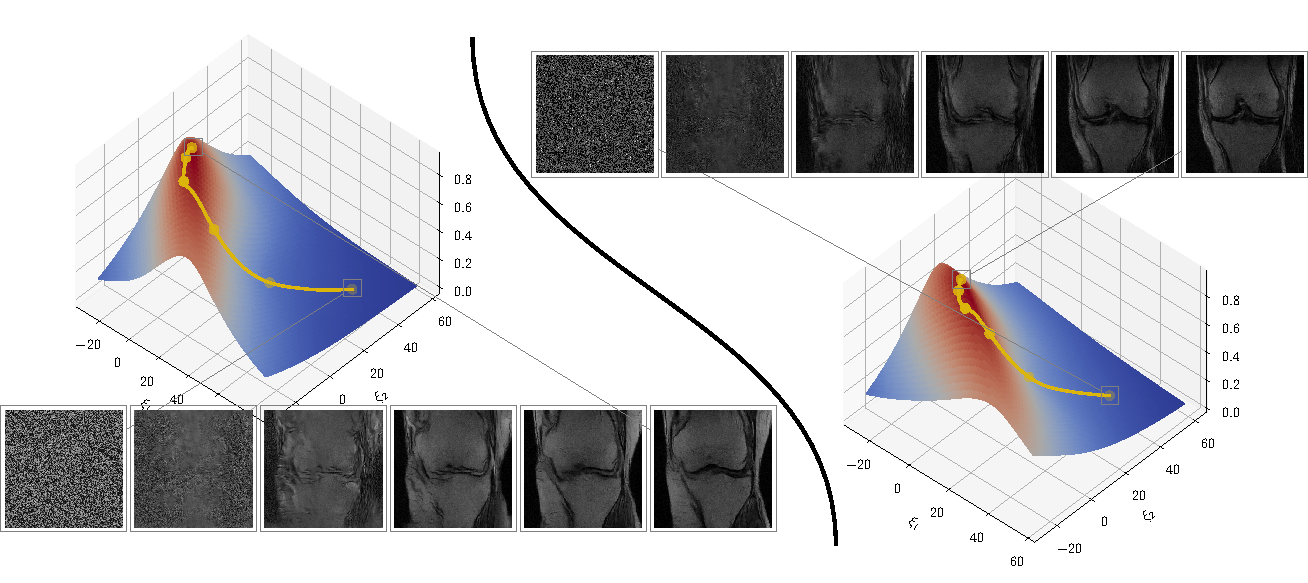
\includegraphics[width=\linewidth]{mri-sampling}
	\caption[Sampling a deep neural regularizer]{%
		We visualize preferred structures of the regularizer via \gls{mcmc} sampling.
		Uniform noise is unlikely under the deep neural regularizer whereas natural anatomical structures are very likely.
		The golden trajectory are the Langevin iterations; see the details in~\cref{ssec:data independent analysis}.
	}%
	\label{fig:mri sampling}
\end{figure*}

The \gls{map} inference problem with the deep neural regularizer is challenging.
The deep neural regularizer is not guaranteed to be convex\footnote{%
	This is somewhat of an understatement, it is almost surely not convex.
} and common neural network activation functions are not differentiable.
Traditional methods handle the non-differentiability is via proximal maps, but computing the proximal map with respect to the neural network is as hard as the original optimization problem, making this approach impractical.

Instead, we rely on nonconvex (nonsmooth) \gls{fista} for optimization, where the gradient step is replaced with a step on the Clarke subgradient (\cref{def:clarke subdifferential}) of the deep neural regularizer.
Specifically, at the point of nondifferentiability of the leaky rectified linear activation (\(\num{0}\)), we choose zero out of the subdifferential.
While we lack theoretical convergence guarantees, empirical results show fast convergence.

We observed that a good initialization is critical, which we achieve by running the optimization algorithm with a slightly noisy signal, matching the noise level used in Langevin iterations during training.see also~\cref{ssec:methods ml}.
Since accelerated algorithms can accumulate errors, we inject noise before gradient and function evaluation, not directly on the optimization variable.
After achieving suitable initialization, we proceed with standard algorithm.
In the resulting algorithm~\cref{alg:nonconvex fista with noise} we chose \( N_\eta = \num{1000} \), \( \gamma_{\num{1}} = \num{2} \), \( \gamma_{\num{2}} = \num{2}/\num{3} \).
After \( N_\eta \) iterations, the algorithm reduces to nonconvex nonsmooth \gls{fista}.
\begin{algorithm}
	\DontPrintSemicolon%
	\SetKwInOut{Input}{Input}
	\Input{Set \( L = \num{1} \), choose initial point \( x_{\num{0}} \in \ImgDim \), number of iterations with noise \( N_\eta \in \mathbb{N} \), noise level \( \epsilon > \num{0} \), backtracking multipliers \( \gamma_{\num{1}} \in \ointerval{1}{\infty}, \gamma_{\num{2}} \in \ointerval{\num{0}}{\num{1}} \).}
	\( x^{-1} = x^{\num{0}} \)\;
	\While{not converged}{
		\( \bar{x}^{k} = x^k + \frac{1}{\sqrt{2}} \bigl( x^k - x^{k-\num{1}} \bigr) \)\;
		\( \eta \sim \NormalDistribution_{\num{0}, \epsilon\Identity} \)\;
		\( \tilde{x}^k = \bar{x}^k + \CharacteristicFunction{\Set{1,\ldots,N_\eta}}(k) \eta \)\;
		\For{ever}{
			\( x^{k+\num{1}} = \prox_{L^{-1}h}\bigl(\bar{x}^k - L^{-1} \Grad g(\tilde{x}^k)\bigr) \)\;
			\uIf{\( g(x^{k+1} + \CharacteristicFunction{\Set{1,\ldots,N_\eta}}(k) \eta) < g(\tilde{x}^k) + \inprod{\Grad g(\tilde{x}^k)}{x^{k+\num{1}} - \bar{x}^k} + \frac{L}{2}\norm{x^{k+1} - \bar{x}^k}_{\num{2}}^{\num{2}}\)}{
				break\;
			}
			\( L = \gamma_{\num{1}}L \)\;
		}
		\( L = \gamma_{\num{2}}L \)\;
		\( k = k + \num{1} \)\;
	}
	\caption{Nonconvex nonsmooth noisy \gls{fista} with backtracking.}%
	\label{alg:nonconvex fista with noise}
\end{algorithm}

The resulting reconstruction shown in~\cref{fig:running example reconstructions/energy-based} is highly satisfactory.
Back-folding artifacts are entirely removed, small anatomical details such as the blood vessels in the fat tissue are restored well.
There are no obvious artifacts and the reconstruction looks natural over all.
In summary, the data-driven deep neural regularizer effectively captures the underlying distribution.
Samples drawn from its Gibbs distribution are almost indistinguishable from reference samples.
This carries over to inverse problem where the regularizer is able to restore anatomical features it has learned from the reference distribution.
Although without theoretical guarantees, the optimization of the deep neural regularizer is straightforward and the resulting images are artifact-free.
\RunningExampleFigure{reconstructions/energy-based}{Data-driven deep regularizer}{Reconstruction using the deep neural regularizer discussed in~\cref{chap:deep neural regularizers}.}

Combining the discussion on decision theory in \cref{chap:intro} with the Bayesian model, we expect that the \gls{mmse} will outperform the \gls{map} estimate.\footnote{At least quantitatively with respect to \gls{psnr}.}
For the sake of simplicity, we do not show \gls{mmse} estimates in this chapter, but quantitative results in~\cref{chap:deep neural regularizers} improve significantly from the \gls{map} estimate to the \gls{mmse} estimate.
\section{Conclusion}
In this section, we reviewed the historical development of regularizers.
Starting with classical methods such as quadratic penalization of gradients, we observed that fitting empirical statistics significantly improves the reconstructions in inverse problems.
The classical anisotropic \gls{tv} regularizer uses the absolute values as the best convex approximation to the empirical marginal distributions of pixel differences.
The nondifferentiability of the \gls{tv} motivated extensive research on nonsmooth optimization, exemplified by the development of the \gls{pdhg} algorithm~\cite{chambolle_primal_2010}.
Compared quadratic gradient penalization, these algorithms offer superior reconstruction quality.

The structure of the \gls{tv} can be viewed as a composition of \emph{prescribed} discrete gradient filters and absolute value potentials.
\emph{Data-driven} regularizers instead learn filters and potentials from a reference distribution.
For (under-)complete models on the space of patches, \gls{pca} provides a suitable filter basis and the optimal potentials can immediately be fit to the empirical marginal distributions.
This richer, data-fitting model outperforms classical TV regularization.

Extending an undercomplete model on image patches to images involves applying the learned filters as convolutions, resulting in an overcomplete model.
A common assumption for natural scenes is translation invariance of their statistics, implying that the potentials should be shared amongst all responses of an image on filter.
Even with shared potentials, the learning problem is significantly more complex.
However, once learned, the model captures richer statistics of the reference distribution.
Recently developed deep neural regularizers further elevate the reconstruction performance.

To conclude the chapter, we summarize the historical development of regularizers in~\cref{fig:running example comparison}.
Our best regularizer improves the naive reconstruction by \qty{5.16}{\decibel} in \gls{psnr}, and improves over anisotropic \gls{tv} regularization by \qty{2.78}{\decibel} in \gls{psnr}.
\begin{figure*}
	\begin{tikzpicture}
		\def\mywidth{4.2cm}
		\def\spywidth{2cm}
		\pgfmathsetlengthmacro{\myhpad}{2 * \spywidth + .8cm}
		\def\myvpad{0.8cm}
		\foreach [count=\imethod from 0] \method/\name/\psnr in {%
			reference-rss/{Reference}/\(\infty\),
			zero-filled/{\( R \equiv 0 \)}/27.94,
			quadratic-intensities/{\( x \mapsto \norm{x}^{\num{2}} \)}/26.76,
			quadratic-gradients/{\( x \mapsto \norm{\DiffOp x}_{\num{2},\num{2}}^{\num{2}} \)}/27.45,
			absolute-gradients/{\( x \mapsto \norm{\DiffOp x}_{\num{1},\num{1}} \)}/30.32,
			patch-prior/{\( x \mapsto \sum_{k=\num{1}}^\NumExperts \Potential_j(\inprod{\Filter_k}{x}) \)}/30.70,
			conv-prior/{\( x \mapsto \sum_{k=\num{1}}^\NumExperts \Potential_j(K_k x) \)}/30.93,
			energy-based/{\( x \mapsto R_\theta(x) \)}/33.10%
		}{%
			\pgfmathsetlengthmacro{\yy}{-abs(\imethod - 3.5) * (\mywidth + \myvpad)}
			\pgfmathsetlengthmacro{\xx}{int(\imethod / 4) * (\mywidth + \myhpad)}
			\pgfmathsetlengthmacro{\yyanno}{\yy - (\mywidth + \myvpad) / 2+0.05cm}
			\pgfmathsetlengthmacro{\xxspy}{\xx + pow(-1, (\imethod > 3)) * (\mywidth + 2cm) / 2}
			\pgfmathsetlengthmacro{\xxpath}{\xx + pow(-1, (\imethod < 4)) * 3cm}
			\ifthenelse{\imethod>0}{\fill (\xxpath, \yy) circle (0.2cm);}{}
			\pgfmathsetlengthmacro{\yypath}{\yy + or(\imethod==3,\imethod==4) * 3cm}
			\coordinate (path\imethod) at (\xxpath, \yypath);
			\begin{scope}[spy using outlines={rectangle, magnification=3, width=\spywidth, height=\mywidth}]
				\node at (\xx, \yy) {\includegraphics[width=\mywidth,angle=180]{reconstructions/\method}};
				\spy [maincolor] on (\xx + 1.5cm, \yy - .3cm) in node at (\xxspy, \yy);
			\end{scope}
			\ifthenelse{\imethod>0}{\node [rectangle, rounded corners, fill=white] at (\xx - 1.6cm, \yy + 1.8cm) {\psnr};}{}
			\node at (\xx, \yyanno) {\name};
		}
		\draw [thick, -latex] \foreach \x [remember=\x as \lastx (initially 1)] in {2,...,7}{(path\lastx) -- (path\x)} (path7) -- ++(0, -1);
	\end{tikzpicture}
	\caption[Running example: Comparison]{%
		The historical development of regularizers:
		\Glsxtrlong{tv} regularization improves over the naive reconstruction (\qty{27.94}{\decibel}) by \qty{2.38}{\decibel}, our best model improves over the \glsxtrlong{tv} regularization by \qty{2.78}{\decibel}.
	}%
	\label{fig:running example comparison}
\end{figure*}
